\section{Obstacle avoidance sensor}
\begin{figure}[H]
    \centering
    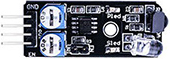
\includegraphics[angle=0, keepaspectratio=true, scale=1, width=200px, height=200px]{images/obstacle_avoidance.jpg}
    %\caption{Caption}
\end{figure}
\subsection*{Description}
The obstacle avoidance sensor works on the same principle as the line tracking sensor module. An infrared transmitter and receiver are placed facing forwards on the module along an on board potentiometer that lets the user adjust the detection range.
\subsection*{Pin mapping}
This pin mapping corresponds to the pins from left to right with the module pins facing towards you.
\begin{table}[H]
    \centering
    \begin{tabular}{|c|c|c|c|c|}
    \hline
    Index &Label &Type &Name &Description\\ \hline
    0 &EN &Unused & &This pin is not used \\ \hline
    1 &VCC &Source voltage &$V+$ &Module source voltage ($5V$)\\ \hline
    2 &OUT &Digital output &D0 &\\ \hline
    3 &GND &Ground &GND &\\ \hline
    \end{tabular}
    %\caption{Caption}
    %\label{tab:my_label}
\end{table}
\subsection*{Operation}
The output voltage at the digital pin (D0) is set to high when the module detects an object. The circuit is completed when the infrared waves emitted from the transmitter and reflected and absorbed by the infrared receiver. As the transmitter and receiver are placed facing forwards on the module, the sensor detects objects in front of the module.

By adjusting the potentiometer on the module the reflectivity threshold can be changed. Note that the potentiometer closest to the ground (GND) pin is factory calibrated and should not be changed.
\subsection*{Code}
Refer to listing \ref{python_avoidance}.